\section{Architecture}
Describe the following:
1. The system must be able to provide a suitable UI for the user, but should not use their computer for anything else 
2. The system must be able to provide some way to execute haskell code and assert whether or not the code is correct. 
3. .... therefore we choose to split the system into multiple subsystem, each being responsible for providing different functionalities to the full system and can run independently of one another. 
4. .... by doing this we gain.....

% Why do we choose the front end we do --- why do we have the 'front end backend?' --- Is the front end system only on the client? No? Why not?

\subsection{Back-end system}
The backend system is responsible for providing the heavy lifting for the other subsystems. %
Some of the responsibilities for this subsystem is persistence of information, authentication of users, and compiling and executing haskell code.

\subsubsection{Code runner}
Our system needs to be able to compile and run haskell code. To accomodate this, a code runner module has been implement in a layered architecture describing the dependencies of components.
Each component can depend only on components on a lower or same level. 
The component is implemented as a HTTP server as seen on Figure \ref{fig:code_runner}.
Whenever the server recieves a HTTP request, a service request is sent to a \textit{code runner} service.
This service in turn writes the content recieved to a Haskell file and invokes the GHC compiler, giving the haskell file as input.
If the compilation of the haskell file fails, the code runner will send the GHC compiler's compilation error as response to the service user.
If the file compiles successfully the code runner will then run the executable file and fetch the produced output of the program.
This output is then sent to the service user.
Finally, the response from the code runner, whether successful or not, is redirected back to the client, providing them with information about the compilation and execution.


\begin{figure}
    \centering
    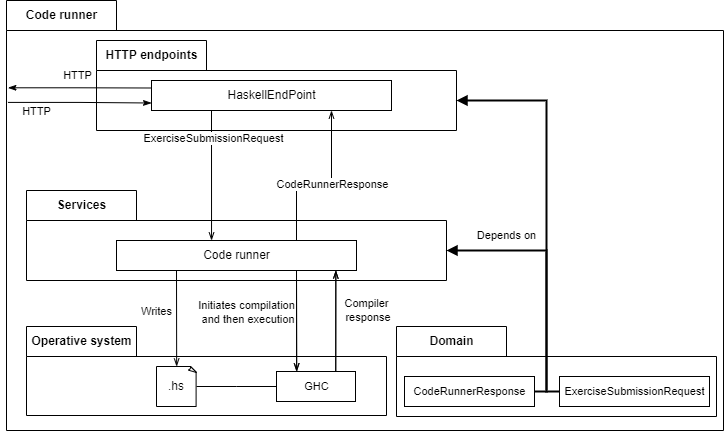
\includegraphics[width=\textwidth,height=\textheight,keepaspectratio]{sections/Chapter 2/pics/P7 arch-Backend - HS compiler.drawio.png}
    \caption[]{The layered architecture of the code runner component for the back end system.}
    \label{fig:code_runner}
\end{figure}

\subsection{Front-end system}

\subsubsection{UI}

\subsubsection{UI business layer}